As part of the CRISP Project, a framework has been developed to test the elaborated change negotiation and propagation algorithms for collaborative processes. The framework already provides functionalities for importing process models in form of BPMN 2.0 XML, deriving public models out of choreography models as well as inserting new fragments into existing models. Within the importing process, the BPMN models are converted into a RPST without loosing any information on the control flow and connection objects of the original model. This resulting graph structure enables model manipulation and analysis techniques. In order to save the effort of implementing the same or similar graph model structure for the automatic process collaboration generator, it was decided to integrate it into the existing framework. Hence, the structure and it's complementary components and services can be utilized with minor adaptations.\par
The following chapter describes the internal process model representation structure and the implemented class structure of the automatic generator and translator.

\section{Internal Process Model Representation}
The framework internal process model representation utilizes the jBPT\footnote{Business Process Technologies for Java - https://code.google.com/p/jbpt/} library, which was developed by Polyvyanyy et. al \cite{jbpt} and facilitates the modeling of process models as RPST. Figure \ref{fig:jbpt} shows an excerpt of the core structure of the library. The structure enables the creation of different types of graphs to support the capturing of various process modeling languages, such as petri nets, EPC\footnote{Event-driven process chains} or BPMN.\par
For the purpose of constructing BPMN process models, an implementation of the \textit{AbstractMultiDirectedGraph} class is suitable. A \textit{multi directed graph} represents a graph whose vertices can be connected among themselves through multiple \textit{directed} edges\cite{graph_theory}. Figure \ref{fig:jbpt} also shows that all graph models are typed with generics. In the context of a \textit{multi directed graph} model, the parameter \textit{E} is bound to a an instance of \textit{IDirectedEdge\textless$V$\textgreater}, whereas parameter \textit{V} is bound to an instance of \textit{IVertex}. 

\begin{figure}[H]
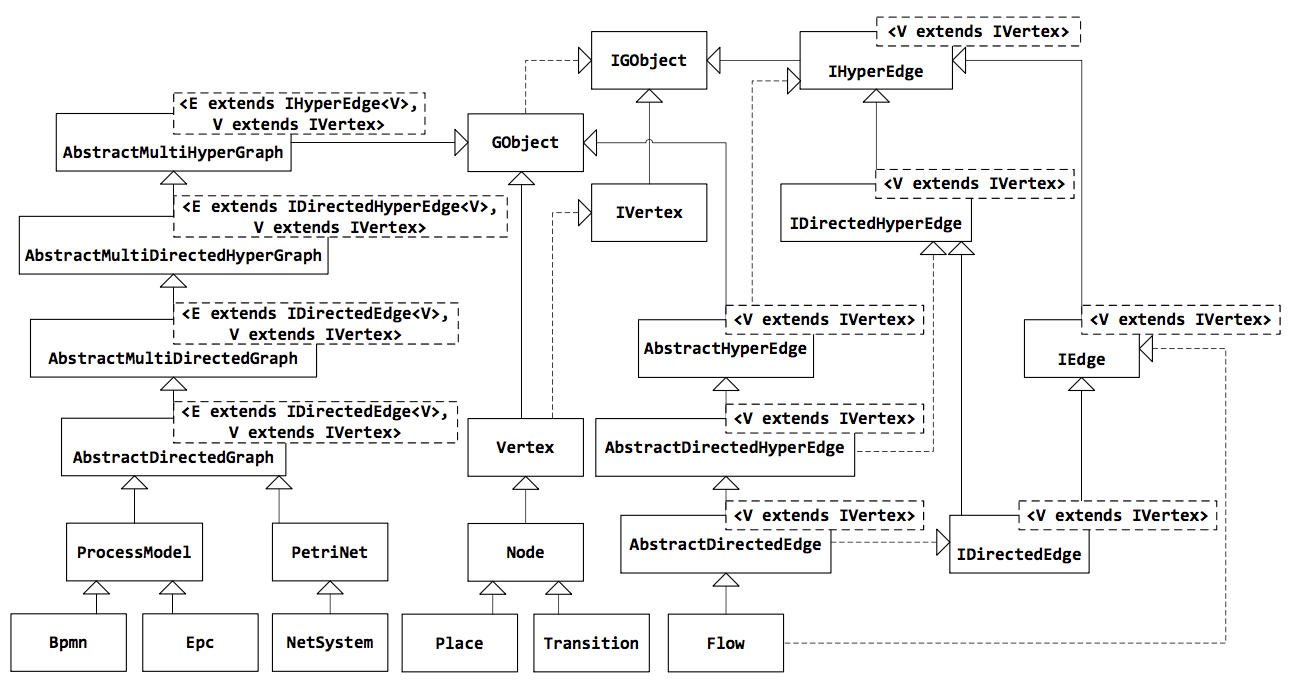
\includegraphics[width=1\textwidth]{src/images/class_diagram_jbpt.png}
\caption{Class and interface hierarchy of jBPT (Source: \cite{jbpt})}
\label{fig:jbpt}
\end{figure}

In order to utilize the jBPT structure to build any type of BPMN process model, all specific BPMN flow objects must therefor implement the \textit{IVertex} interface. The flow objects, for instance tasks or gateways, are then in turn connected through Edges, which represent the BPMN sequence flow to create the graph and therefor the process model. How the jBPT library is incorporated and utilized by the framework is illustrated in figure \ref{fig:choreo_structure}. 
The intensive use of interfaces enables the reuse of flow objects that are part of different model types. For instance, gateways and events are used in all four model types. For the sake of clarity, Figure \ref{fig:choreo_structure} only shows model specific flow objects that are appropriate for BPMN choreography models. Table \ref{tab:flow_objects} lists all BPMN flow objects, that are supported by the framework to create process collaborations and their different models.\\

\begin{table}[H]
\resizebox{\textwidth}{!}
{
\begin{tabular}{l|cccc}
			      & Choreography Model & Collaboration Model & Public Model & Private Model \\ \hline
Start Event       & $\blacksquare$	  & $\blacksquare$      & $\blacksquare$	  & $\blacksquare$  \\
End Event         & $\blacksquare$	  & $\blacksquare$      & $\blacksquare$	  & $\blacksquare$  \\
Parallel Gateway  & $\blacksquare$    & $\blacksquare$      & $\blacksquare$      & $\blacksquare$  \\
Exclusive Gateway & $\blacksquare$    & $\blacksquare$      & $\blacksquare$      & $\blacksquare$  \\
Interaction       & $\blacksquare$    & $\square$           & $\square$           & $\square$       \\
Task          	  & $\square$         & $\blacksquare$      & $\blacksquare$      & $\blacksquare$  \\
Send Task         & $\square$         & $\blacksquare$      & $\blacksquare$      & $\blacksquare$  \\
Receive Task      & $\square$         & $\blacksquare$		& $\blacksquare$      & $\blacksquare$       
\end{tabular}%
}
\caption{Overview of supported BPMN flow objects}
\label{tab:flow_objects}
\end{table}

Within the framework, all four model types support the flow objects \textit{Start Event, End Event, Parallel Gateway} and \textit{Exclusive Gateway}. These are basic control flow objects that are not specific to any model type in BPMN. Additionally available, for \textit{collaboration, public} and \textit{Private Models}, are the activities \textit{Task, Send Task} and \textit{Receive Task}. According to the BPMN 2.0 specification, the activity \textit{Task} represents an \textit{Abstract Task} \cite{BPMN20}. An \textit{Abstract Task} is a task that is not further specified. There are several further specified tasks in BPMN, including the also supported \textit{Send} and \textit{Receive Task}. Since the focus of the CRISP project is on collaborative processes and the message exchange between the participating partners, it is mandatory that these two messaging activities are also specified within the framework. For the remaining activities that are not part of the message flow, it is in this context not relevant if the task is actually a \textit{User, Manual, Service} or \textit{Script task}. The only flow object specific for \textit{Choreography Models} is the \textit{Choreography Task} or \textit{Interaction}, the equivalent of a \textit{Send} and \textit{Receive task} sequence in a collaboration model.   

\begin{figure}[H]
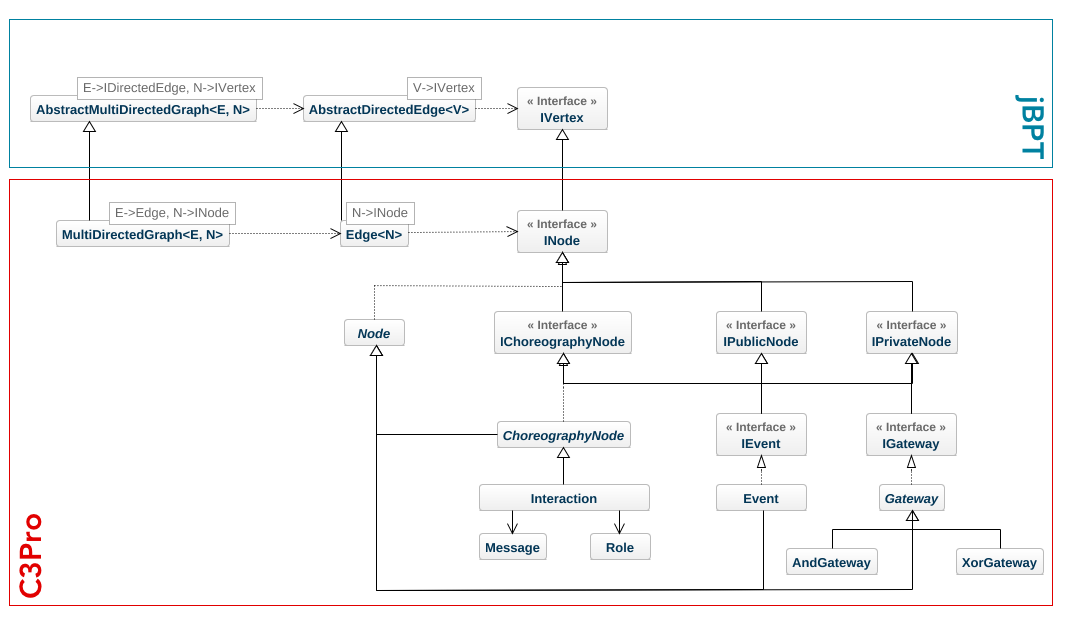
\includegraphics[width=1\textwidth]{src/images/c3pro_graph_structure.png}
\caption{Framework Model Representation Structure}
\label{fig:choreo_structure}
\end{figure}

\section{Class Structure and Data Model}

The diagram shown in Figure \ref{fig:impl_class_overview} represents the simplified class structure of the implemented components, that are necessary for generating an entire process collaboration, starting with the generation of the Choreography Model that complies to imposed compliance rules, leading to deriving the Public and Private Models out of it and finishing with the translation to BPMN/XML. The numbers indicate the order in which the components are instantiated. In the following, each class, their core functions and their relation with to the algorithms, introduced in the section of conception, will be described.

\begin{figure}[H]
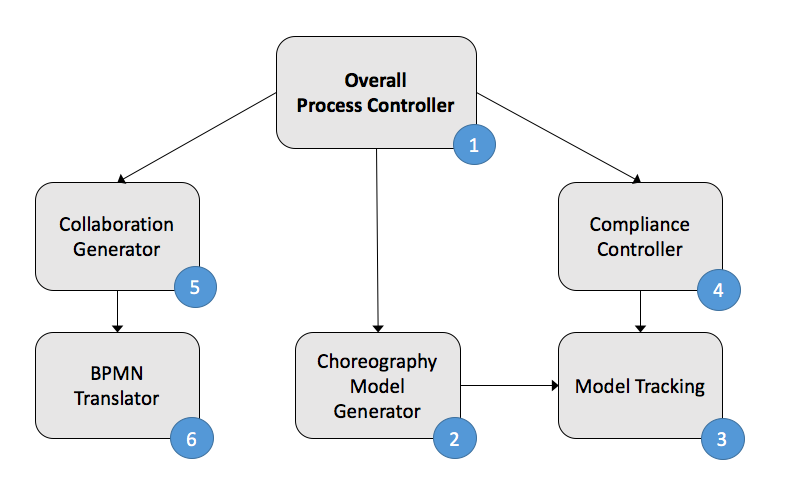
\includegraphics[width=1\textwidth]{src/images/impl_architecture.png}
\caption{Class Structure Random Collaboration Generator}
\label{fig:impl_class_overview}
\end{figure}

The logic of coordinating the entire generation process (see Algorithm \ref{alg:choreographyController}) is implemented in the class \textit{CollaborationGenerationController}. It's purpose is to orchestrate the whole process and functionalities provided by the other components. Also the parametric build constraints and compliance rules, on which the collaboration generation is based, are specified within this class.\\

The class \textit{ChoreographyModelGenerator} encapsulates the functionality of generating a random choreography model. Figure \ref{fig:impl_chormodelgen_overview} shows the extended class structure of the \textit{Choreography Model Generator} component and the important instance variables and implemented methods of each class. The main class of this component is the \textit{ChoreographyModelGenerator} class. Within this, the algorithm for generating random models, explained in the chapter of conception (see Algorithm \ref{alg:choreoGen}), is implemented within the \textit{build()} method. The thereby used functions \textit{getRandomNodeType()} (see Algorithm \ref{alg:randNodeType}), \textit{getRandomBranch()} (see Algorithm \ref{alg:randBranch}) and \textit{getRandomBranchAmount()} are also implemented within this class, whereby all utilize methods that are implemented within the \textit{ModelTracking} class. This includes mainly methods for updating the model and determining the amount of free and reserved interactions. Within the \textit{ModelTracking} a set of splits is contained which represents the actual model as branches and associated nodes. The different node types all implement the \textit{IChoreographyNode} interface. 

\begin{figure}[H]
\centering
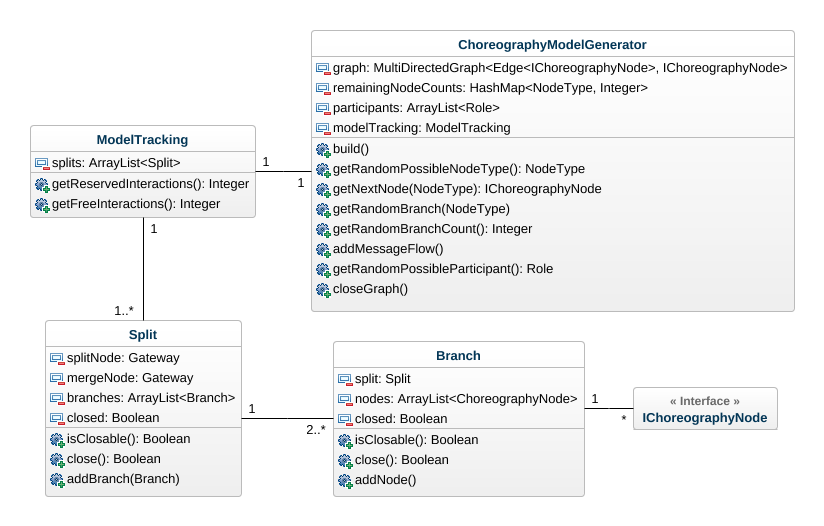
\includegraphics[width=0.8\textwidth]{src/images/chormodelgenerator_class.png}
\caption{Class Structure - ChoreographyModelGenerator}
\label{fig:impl_chormodelgen_overview}
\end{figure}

The introduced logic of specifying and imposing global compliance rules on a choreography model is implemented within the class \textit{ComplianceController}. It also utilizes the same instance of the \textit{ModelTracking} class, that represents the finished model in order to find possible assignments for the imposed interaction order.\\

\begin{figure}[H]
\centering
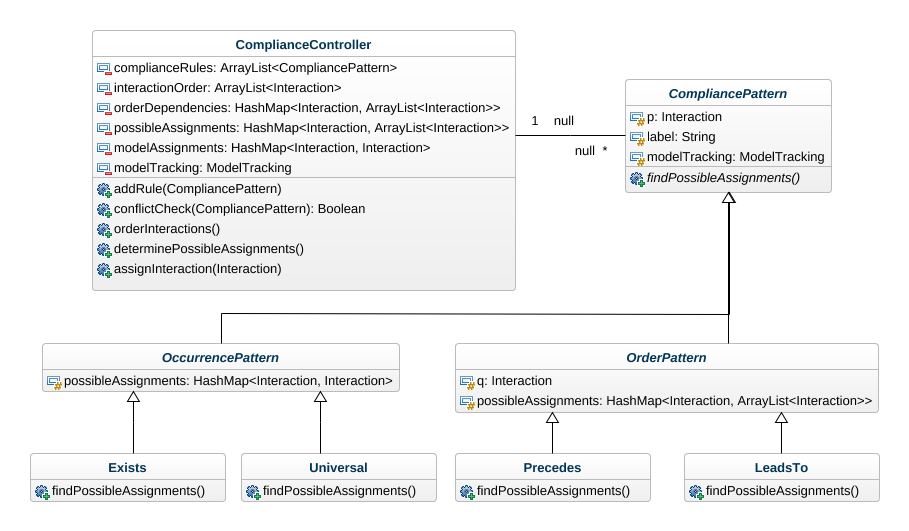
\includegraphics[width=0.8\textwidth]{src/images/compliancecontroller_class.png}
\caption{Class Structure - ComplianceController}
\label{fig:impl_compcon_overview}
\end{figure}

Figure \ref{fig:impl_compcon_overview} represents the class class diagram of the implemented component. Within the \textit{ComplianceController} class, the procedure for conflict checking between the specified rules (see Algorithm \ref{alg:conflictCheck}) is implemented by the \textit{conflictCheck(CompliancePattern)} method. The \textit{assign()} method orchestrates the whole assignment process by fist triggering the \textit{findPossibleAssigment()} method of each involved compliance pattern by calling the \textit{determinePossibleAssignments()} method. The \textit{findPossibleAssigment()} methods determines the possible model positions for each pattern type individually based on the rules described in Definitions \ref{def:leadsto} - \ref{def:exists}. In the next step, the order of involved interactions is determined by the \textit{orderInteractions()} method. Based on the resulting order, the interactions are tried to be assigned into the choreography model by the \textit{assignInteraction(Interaction)} method (see Algorithm \ref{alg:imposecr}).\\

The class \textit{CollaborationGenerator} provides the functionalities of deriving the public and private models from the generated choreography model. This component is already implemented within the framework and is therefor not described as a part of the implementation.\\

At last, the translation of the internal model representation to BPMN/XML, based on the mappings described in Section \ref{sec:bpmntranslation} of the conceptional chapter, is implemented within the \textit{BPMNTranslator} class. The process is a typical XML generation process, utilizing the established jDOM\footnote{Java library for XML manipulation} library.

\section{Conclusion}
In this chapter, the internal model representation and the therefore utilized jBPT library was explained. It was shown how the provided \textit{AbstractMultiGraph} and its data model is extended in order to meet the requirements of BPMN choreography models. The chapter was concluded with an overview of how the different components are implemented within the existing framework and by linking the important methods with the algorithms introduced within the chapter of conception. In the next chapter, the implementation of the choreography generation process is examined by analyzing the performance and the resulting models based on different parameter settings. 
